%!TEX root = report.tex

Einstein's theories of relativity make bold claims about the nature of reality, and after they were published physicists were immediately interested in verifying the claims made by the theory experimentally. In this chapter we will present the three ``classical'' tests of general relativity, which were the first tests to be done after Einstein published his theories. These observations are made on bodies within our solar system, and mostly use the Schwarzschild metric obtained at the end of the first chapter.

\section{The Precession of Mercury's Perihelion}

Celestial mechanics based on Newtonian gravitational theory had been incredibly successful in describing the motion of the planet's within the solar system. There was one exception to this however: the precession of Mercury's perihelion. The perihelion is defined to be the point of a planets orbit within an ellipse which is closest to the sun \cite{cheng}. Over time, the axis of the ellipse of the orbit moves. This is mostly due to the gravitational effects of the other planets in the solar system. However, when such effects are taken into account, there is still a precession of 43 arcseconds per century.

This effect had been observed around about 1850 by astronomers, and many had tried and failed to explain this additional precession of Mercury's orbit; for example by postulating the existence of a smaller planet between Mercury and the sun. It was only after general relativity had been formulated that we can explain this additional contribution to the precession \cite{cheng}.

In order to derive this effect we require the orbital equations derived from the Schwarzschild metric \eqref{schwarzschild} using Lagrangian mechanics. We choose the Lagrangian for a particle in a gravitational field modeled by the Schwarzschild metric to be \cite{cheng}
\begin{equation} \label{schwarzschild-lagrangian}
	\mathcal{L} = \left(\frac{ds}{d\tau}\right)^2 = g_{\mu \nu} \dot{x}^{\mu} \dot{x}^{\nu}
\end{equation}
where we choose \(\tau\) to be the proper time and \(\dot{x}\) is the derivative with respect to the proper time. We recall from classical mechanics that a constant of motion will be the case when \cite{mech}
\begin{equation} \label{lagrangian-constant}
	\frac{\partial \mathcal{L}}{\partial x^{i}} = 0
\end{equation}
for a particular coordinate \(x^{i}\). In the case of the Schwarzschild metric we apply these to \(t\) and to \(\phi\) \cite{hartle}
\begin{equation} \label{conservation}
	\begin{aligned}
		\frac{d}{d \tau} \left(\left(1 - \frac{2 G M}{r}\right) \frac{dt}{d \tau}\right) &= 0 \\
		\frac{d}{d \tau} \left(r^2 \frac{d \phi}{d \tau}\right) &= 0
	\end{aligned}
\end{equation}
and find that those coordinates are constant in time. For the time coordinate, this corresponds to conservation of energy and we will give this constant the symbol \(E\) \cite{hartle, carroll}. For the \(\phi\) coordinate this corresponds to conservation of angular momentum \cite{hartle} which we will call \(L\). 

By recalling from special relativity that \(ds^2 = - d \tau^2\) we can write the Lagrangian in the Schwarzschild case for massive particles as \cite{cheng}
\begin{equation} \label{schwarzschild-lagrangian2}
	\mathcal{L} = - \left( 1 - \frac{2 G M}{r}\right) \dot{t}^2 + \left(1 - \frac{2 G M}{r} \right)^{-1} \dot{r}^2 + r^2 \dot{\phi}^2 = -1
\end{equation}
where we set \(\theta = \frac{\pi}{2}\) as the orbits will always stay in that plane.

Now, by putting \(E\) and \(L\) into the Lagrangian \eqref{schwarzschild-lagrangian2} we can obtain
\begin{equation} \label{energy-balence}
	- \frac{E^2}{1 - 2GM/r} + \frac{\dot{r}^2}{1 - 2GM/r} + \frac{L^2}{m^2 r^2} = -1
\end{equation}
with \(m\) the mass of the particle. Then, if we multiply by \(\frac{1}{2} m (1 - 2GM/r)\) and rearrange we find
\begin{equation} \label{energy-balence2}
	\frac{1}{2} m \dot{r}^2 + \left( 1 - \frac{2GM}{r}\right) \frac{L^2}{2mr^2} - \frac{GmM}{r} = \frac{m E^2}{2} - \frac{1}{2} m
\end{equation}

Now, if we define a new constant \(\mathcal{E}\) to be
\begin{equation} \label{weird-E}
	\mathcal{E} = m \frac{E^2 - 1}{2}
\end{equation}
we can rewrite \eqref{energy-balence2} to be in the form of a Newtonian energy balance equation \cite{cheng}
\begin{equation} \label{energy-balence3}
	\frac{1}{2} m \dot{r}^2 + \left( 1 - \frac{2 G M}{r}\right) \frac{L^2}{2mr^2} - \frac{G m M}{r} = \mathcal{E} .
\end{equation}

At this point it is possible to formulate an orbital equation for Mercury in terms of \eqref{energy-balence3} however we will not do so, and simply state the result. If we define \(e\) to be the eccentricity of the orbit, \(\alpha = L^2 / GMm^2 = (1+e)r_{\text{min}}\) with \(r_{\text{min}}\) the radial distance at the perihelion and \(\epsilon = 6GM/2\alpha\) then the radius of the planets orbit will be given by
\begin{equation} \label{perihelion}
	r = \frac{\alpha}{1 + e \cos ((1 - \epsilon) \phi)} .
\end{equation}
We can see that this will not return to the same point after 1 orbit (when \( \phi = 2 \pi\)), but after slightly greater than one orbit (when \(\phi = 2 \pi / (1 - \epsilon)\)). The entire orbit will advance per revolution by
\begin{equation} \label{perihelion-advance}
	\delta \phi = \frac{6 \pi G M}{(1 - \epsilon) r_{\text{min}}} .
\end{equation}

We now input the values we know for the quantities: the Schwarzschild radius of the sun is \(2GM = 2.95\)km, Mercury's eccentricity is \(e = 0.206\) and the perihelion is at \(r_{\text{min}} = 4.6 \times 10^{7}\)km \cite{cheng} then we can get the numerical value of the advance per revolution as
\begin{equation} \label{perihelion-solved}
	\delta \phi = 5 \times 10^{-7} \, \, \text{radians per revolution}
\end{equation}
which we then can convert to arcseconds per century to get 43 arcseconds per century, in perfect agreement with observations. 
\section{Deflection of Light by the Sun}

In 1919, Arthur Eddington observed a star on the edge of the sun as a solar eclipse was occurring. This star was actually behind the sun, and the light from the star was being bent by the gravitational field of the sun. This provided the second experimental test of general relativity, the effect of gravity on light rays.

Recall from chapter 2 that light travels on a light like world line, with \(ds^2 = 0\). If we choose this direction to be along the coordinates such that \(\phi = \theta = 0\) then the metric will take the form \cite{cheng}
\begin{equation} \label{light-bend-metric}
	ds^2 = g_{00} c^2 \text{d}t^2 + g_{rr} \text{d}r^2 = 0
\end{equation}
where we include the speed of light term for clarity in the following steps.

From this metric we can find the effective speed of light that an observer sees \cite{cheng}
\begin{equation} \label{speed-bending}
	c (r) = \frac{dr}{dt} = c \sqrt{- \frac{g_{00} (r)}{g_{rr} (r)}} .
\end{equation} 
If we now note from the Schwarzschild metric \eqref{schwarzschild} that \(g_{rr} = - (g_{00})^{-1}\) then we can define an index of refraction for the observer by
\begin{equation} \label{light-bend-refraction}
	n(r) = \frac{c}{c(r)} = \sqrt{- \frac{g_{rr} (r)}{g_{00} (r)}} = \frac{1}{- g_{00} (r)} = \left(1 - \frac{2 G M}{r c^2}\right)^{-1} .
\end{equation}

If we now consider a light wave propagating along the \(x\) axis with the gravitational field along the \(y\) axis then a section of the wave front which is closer to the source will travel more slowly than a section further from the source. The amount of this bending, given in terms of a deflection angle from the straight path the light would take without gravity, is given by \cite{cheng}
\begin{equation} \label{bending}
	\delta \phi = \frac{4 G M}{c^2 r_{\text{min}}}
\end{equation}
where in this case \(M\) is the solar mass and \(r_{\text{min}}\) is the closest that the light comes to the large object bending it.

For the test that Eddington performed this resulted in a deflection of \(1.74\) arcseconds, which is exactly what was observed.

A more modern test of this phenomena is looking for gravitational lensing of very distant objects by massive objects in between. A lens equation for light bending is
\begin{equation} \label{lens}
	\beta = \theta - \frac{D_{ls}}{D_{s} D_{l}} \frac{4 G M}{\theta c^2}
\end{equation}
with \(\beta\) the angle from the real object to the observer, \(\theta\) the angle from the image to the observer, \(D_{sl}\) the distance from the source to the mass causing deflection, \(D_{s}\) the distance from source to observer and \(D_{l}\) the distance from the mass to the observer. 

Such events produce Einstein rings in the special case when \(\beta = 0\), that is the source, the massive object acting as a lens and the observer are all aligned. The angular radius in this case will be
\begin{equation} \label{angular-radius}
	r_{A} = \sqrt{ \frac{D_{ls}}{D_{s} D_{l}} \frac{4 G M}{c^2}} .
\end{equation}

Thus we see how astronomers can use gravitational lensing observations to ``weigh'' objects which act as the lens, such as a blackhole which lenses an object at a known distance.

\begin{figure}[h!]
	\centering
	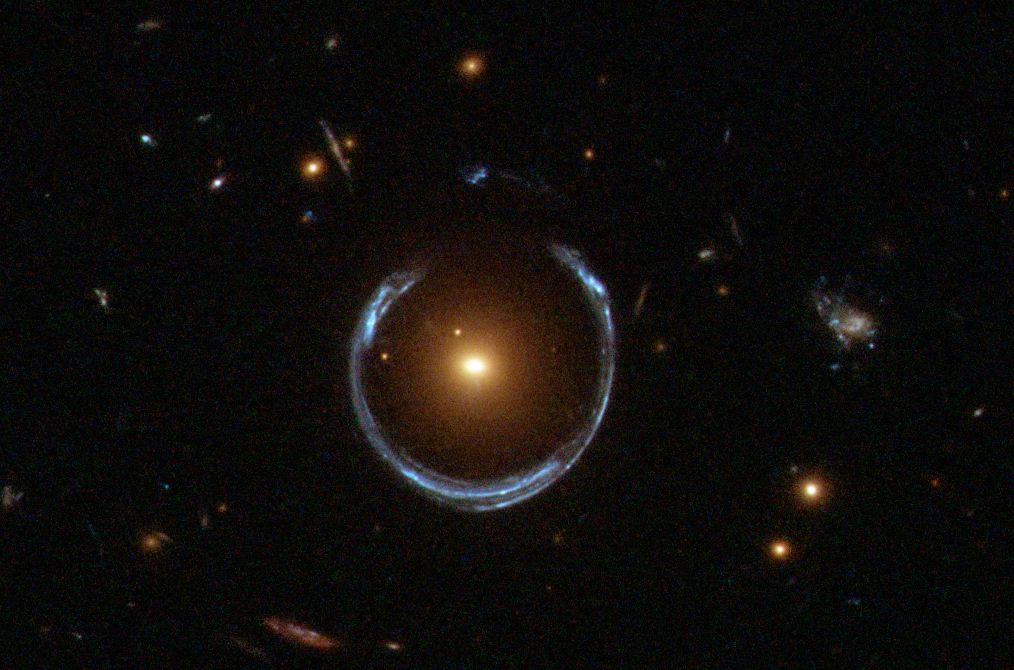
\includegraphics[scale=0.59]{ering.jpg}
	\caption{A picture of an Einstein ring taken by the Hubble space telescope. Light from the blue galaxy is bent by the red galaxy in the foreground.}
\end{figure}

\section{Gravitational Redshift}

Gravitational redshift is an effect where light emitted closer to a large object will appear redshifted when viewed further from that object. It is caused by gravitational time dilation, as frequency is a time based phenomena.

In order to derive the effect, consider an observer who is stationary in a Schwarzschild spacetime. For this observer \(U^{i} = 0\) that is, the spatial part of the four velocity is zero. Thus, because for objects with mass we must have \(U_{\mu} U^{\mu} = -1\) we can get \(U^{0}\) \cite{carroll}
\begin{equation} \label{time-dilation-schwarzschild}
	U^{0} = \left( 1 - \frac{2 G M}{r}\right)^{- \frac{1}{2}} .
\end{equation}

This observer will measure the frequency of the photon along a null geodesic as
\begin{equation} \label{photon-null-geodesic}
	\omega = - g_{\mu \nu} U^{\mu} \frac{d x^{\nu}}{d \lambda} .
\end{equation}

Now in terms of \(U^0\) this relation is \cite{carroll}
\begin{equation} \label{frequency}
	\omega = \left(1 - \frac{2 G M}{r}\right)^{\frac{1}{2}} \frac{dt}{d \lambda} .
\end{equation}
If we now substitute for the definition of \(E\) from \eqref{conservation} then we will find
\begin{equation} \label{frequency2}
	\omega = \left( 1 - \frac{2 G M}{r} \right)^{-\frac{1}{2}} E
\end{equation}
where we take \(E\) to be defined in terms of the affine parameter \(\lambda\) for light. From this we can see that \(\omega\) will take different values depending only on the radius, as \(E\) is conserved throughout the path. If we recall that the radial coordinate is measured by spheres from the source of gravitation we see that the effect is dependent on the photon's height in the gravitational potential, as we expected \cite{carroll}. 

For a photon emitted at \(r_1\) and observed at \(r_2\) we can take the ratio of values of \eqref{frequency2} to obtain the frequency shift
\begin{equation} \label{frequency-ratio}
	\frac{\omega_2}{\omega_1} = \left( \frac{1 - 2GM/r_{1}}{1 - 2GM/r_{2}}\right)^{\frac{1}{2}} .
\end{equation}
Now, if we consider the case where \(r >> 2GM\) we can give a useful approximation
\begin{equation} \label{frequency-shift-approx}
	\frac{\omega_2}{\omega_1} = 1 - \frac{GM}{r_1} + \frac{GM}{r_2} = 1 + \Phi_1 - \Phi_2
\end{equation}
where \(\Phi = -GM / r\) is the Newtonian potential.

The experiment to test these predictions was the last of the classical tests of general relativity, and is called the Pound-Rebka experiment. In 1959, Robert Pound and his PhD student Glen Rebka suggested that it would be possible to measure the gravitational redshift of light on earth \cite{poundrebka}. By accounting for the special relativistic frequency shift of
\begin{equation} \label{special-rel-frequency}
	f = \sqrt{\frac{1 - v}{1 + v}} f_{0}
\end{equation}
which is contrary to the effects of gravitational frequency shifts, it would be possible to measure the effects of light falling down the elevator shaft in Harvard university's physics building \cite{poundrebka}. By moving the apparatus upwards away from the receiver at the bottom of the elevator shaft the effects of \eqref{special-rel-frequency} and \eqref{frequency-ratio} could be balanced, allowing Pound and Rebka simply to observe a signal at exactly the same frequency as the emitted signal.

In order to do this Pound and Rebka had to rely on very high frequency gamma waves, as otherwise it would have been impossible to detect the very small frequency shift due to the change in gravitational potential. Additionally, they had to use a specific crystal structure for the gamma source, in order to reduce the recoil of the atom within the source during the emission of the gamma rays which would cause additional Doppler effects which would be difficult to measure consistently.

The Pound Rebka experiment was highly successful test of general relativity's predictions, and later experiments using similar techniques would bring the error bounds to less than 1\% of the expected values \cite{lrr-2006-3}.